\documentclass{article}
\usepackage{graphicx}
\usepackage{wrapfig}
\usepackage{subcaption}
\usepackage[margin=1in]{geometry}
\usepackage{amsmath} % or simply amstext
\usepackage{siunitx}
\usepackage{booktabs}
\usepackage[export]{adjustbox}
\newcommand{\angstrom}{\textup{\AA}}
\newcommand{\colormap}{jet}  % colorbar to use
\usepackage{cleveref}
\usepackage{booktabs}
\usepackage{gensymb}
\usepackage{float}
\usepackage{hyperref}
\title{Simulated Structure Factors}
\author{Benjamin J. Coscia}
\begin{document}
  \bibliographystyle{ieeetr}
  \graphicspath{{./figures/}}
  \maketitle

  \section{Calculation of the structure factor}

  The structure factor, S($\mathbf{q}$), relates the observed intensity per
  atom to that observed by a single scattering unit. Incident plane waves falling
  on a material have a wave vector, $K_i$, whose length is
  $\dfrac{2\pi}{\lambda}$, where $\lambda$ is the wavelength. The diffracted wave
  vector, $K_f$, has the same length as $K_i$ if the diffraction process is 
  elastic. We will assume elasticity going forward. The scattering vector, $\mathbf{q}$
  is defined as $K_f - K_i$. Since $K_f$ and $K_i$ are the same length, the scattering
  vector must lie on the surface of a sphere of radius $\dfrac{2\pi}{\lambda}$. This
  sphere is called the Ewald Sphere and diffraction will only occur for reciprocal
  lattice points that lie on its surface. 

  The amplitude and phase of the scattered waves is the vector sum of all scattered 
  waves from all atoms:
  \begin{equation}
  \Psi_s(\mathbf{q}) = \sum_{j=1}^{N}f_je^{-i\mathbf{q}\boldsymbol{\cdot}\mathbf{R_j}}\label{eqn:dft}
  \end{equation}
  where $f_j$ is the atomic form factor of atom $j$ and $\mathbf{R_j}$ is the position of
  the atom in real space. Note that Equation \ref{eqn:dft} is the definition of the 
  discrete fourier transform.

  The scattered intensity is obtained by multiplying Equation \ref{eqn:dft} by its 
  complex conjugate:
  \begin{equation}
  I(\mathbf{q}) = \Psi_s(\mathbf{q})\cdot\overline{\Psi_s}(\mathbf{q}) = \sum_{j=1}^{N}f_je^{-i\mathbf{q}\boldsymbol{\cdot}\mathbf{R_j}} \times \sum_{k=1}^{N}f_ke^{-i\mathbf{q}\boldsymbol{\cdot}\mathbf{R_k}} = \sum_{j=1}^{N}\sum_{j=k}^{N}f_jf_ke^{-i\mathbf{q}\boldsymbol{\cdot}(\mathbf{R_j}- \mathbf{R_k})}
  \label{eqn:conjugate}
  \end{equation}
  Computationally, one should calculate the fourier transform of the atomic
  coordinates with a fast fourier transform, calculate its complex conjugate and 
  multiply them together. The structure factor is typically normalized as 
  $ 1 / {\sum_{j=1}^{N} {f_j}^2}$ so that it is independent of system size, and
  the general equation for the structure factor becomes:
  \begin{equation}
  S(\mathbf{q})= \dfrac{1}{\sum_{j=1}^{N} {f_j}^2}\sum_{j=1}^{N}\sum_{j=k}^{N}f_jf_ke^{-i\mathbf{q}\boldsymbol{\cdot}(\mathbf{R_j}- \mathbf{R_k})}
  \label{eqn:general_sf}
  \end{equation}
 
  If all atoms are identical, equation \ref{eqn:general_sf} simplifies to:
  \begin{equation}
  S(\mathbf{q})= \dfrac{1}{N}\sum_{j=1}^{N}\sum_{j=k}^{N}e^{-i\mathbf{q}\boldsymbol{\cdot}(\mathbf{R_j}- \mathbf{R_k})}
  \label{eqn:simplified_sf}
  \end{equation}

  The atomic form factor, $f_j$ is more complicated than how it is represented
  in Equation \ref{eqn:dft}. The atomic form factor is the scattering
  contribution from a single isolated atom. They are calculated as the fourier
  transform of the electron density, $\rho({\mathbf{r}})$,  which is typically
  calculated using quantum techniques. Since $\rho({\mathbf{r}})$ is a spatially
  dependent function, $f_j$ is actually a function of $\mathbf{q}$,
  $f(\mathbf{q})$. Values of $f(\mathbf{q})$ for each element are tabulated in
  the \href{http://it.iucr.org/Cb/ch6o1v0001/}{International Tables for
  Crystallography}. For $\mathbf{q}=\mathbf{0}$, the atomic form factor is equal to the 
  number of electrons possessed by the atom. 

  The resolution in each dimension of reciprocal space is determined by the
  size of the unit cell studied. In order to calculate the structure factor, the
  system's 3D coordinates must be discretized into regularly sampled points using
  a histogramming method. Applying equation~\ref{eqn:general_sf} to the histogram
  will yield a grid with Fourier bin sizes of $\dfrac{2\pi}{L_i}$ (i = (x,y,z)).
  The fourier transform of an array of values returns a same length array of
  frequencies. Increasing the number of bins in the histogram will not change the
  size of the Fourier space bins, rather it will increase the maximum accessible
  value of $q$. 

  \section{Structure factor of hexagonally packed columns}

  Here, we explore, in depth, a simplified model of an inverted hexagonal phase
  lyotropic liquid crystal (H\textsubscript{II} LLC). The simplified model is
  meant to enhance our understanding of the structure factor of a fully atomistic
  model of the same material. We are primarily interested in the diffraction
  patterns produced by the head groups so we model each monomer as a point placed
  at the center of mass of its head group. The hexagonal phase is made up
  straight pore columns. Each pore column is composed of columns of stacked
  monomers which surround the pore's hydrophilic core. Based on simulation, there
  are likely 5 monomer columns making up each pore, and the pore radius is ca. 1
  nm. Experimental WAXS suggests that monomers stack 3.7 \AA apart, and SAXS
  measurements have shown that pores are spaced ca. 4.1 nm apart. Here we took the 
  pore spacing to be 4.25 nm for no good reason. For consistency with simulation,
  we will look at 4 pores in a monoclinic unit cell with 5 monomer columns per pore. 

  We are interested in the intensity and dimensions of the R-$\pi$ reflection,
  which is a consequence of monomers stacked on top of each other in the
  z-direction.

  \subsection{Crystalline liquid crystals}

  For a perfect, infinite crystal, the intensity of R-$\pi$ is infinitely sharp. We
  created a model with perfectly aligned columns. Each columns originates at z=0
  and all other points in the column are equally spaced 3.7 \AA apart in the
  z-direction (Figure~\ref{fig:perfect_crystal_xyz}). This essentially creates
  layers of atoms. The intensity of R-$\pi$ for systems of various size are shown
  in Table~\ref{table:perfect_size_dependence}. The intensity of R-$\pi$ is equal
  to the number of atoms in the unit cell. The intensity will approach infinity as
  the system size increases.  

  \begin{figure}[!htb]
  \centering
  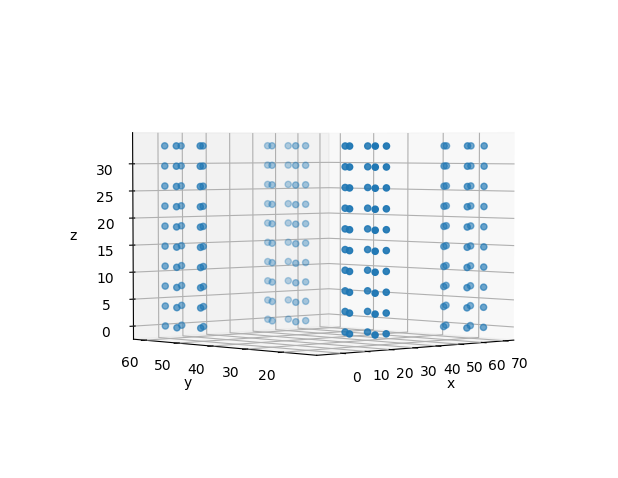
\includegraphics[width=0.5\textwidth]{perfect_crystal_xyz.png}
  \caption{}\label{fig:perfect_crystal_xyz}
  \end{figure}

  \begin{table}
  \centering
  \begin{tabular}{c c c c c c}
  \toprule
  $L_z$ (\AA) & Points per column & Number of Pores &  Number of Atoms & R-$\pi$ Intensity & FWHM ($\AA^{-1}$) \\
  \midrule
  14.8        &      4            &       4          & 80               & 80               & 0.34  \\
  18.5        &      5            &       4          & 100              & 100              & 0.34  \\
  37          &      10           &       4          & 200              & 200              & 0.34  \\
  14.8        &      4            &       9          & 180              & 180              & 0.36  \\
  18.5        &      5            &       9          & 225              & 225              & 0.36  \\
  37          &      10           &       9          & 450              & 450              & 0.36  \\
  14.8        &      4            &       16         & 320              & 320              & 0.43  \\
  18.5        &      5            &       16         & 400              & 400              & 0.43  \\
  37          &      10           &       16         & 800              & 800              & 0.43  \\
  \bottomrule
  \end{tabular}
  \caption{The intensity of R-$\pi$ in a perfect crystal is equal to the number of
  scatterers in the unit cell.}\label{table:perfect_size_dependence}
  \end{table}

  We measured the peak width of R-$\pi$ in the $q_r$ direction using the
  appropriate slice of the structure factor. Ideally, one should use the angle
  averaged structure factor for this calculation, but since the angle averaging
  procedure interpolates between bins, the averaged intensities are lower than
  expected which slightly changes the shape of the peak. This reflection is
  radially symmetric about the z-axis, so we fit peak widths to cross-sections at
  (0, y, 1.7)$^{-1}$ \AA. 

  The distance, d, between peaks in the $q_y$ cross-sections of the structure
  factor is equal to $2\pi / d$ (Figure~\ref{fig:p2p_rpi}). We looked at systems
  with pores spaced 42.5 nm and 212.5 nm apart respectively.  The fundamental
  frequency appears where expected, based on d. Subharmonics follow the
  fundamental frequency at equally spaced intervals of width $2\pi / d$. 

  \begin{figure}[!htb]
  \centering
  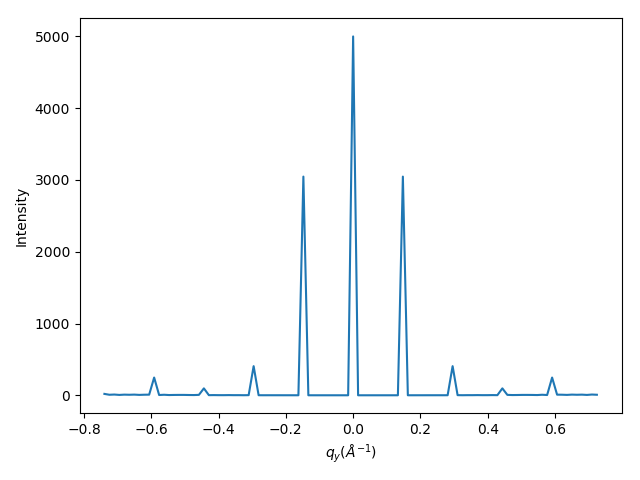
\includegraphics[width=0.45\textwidth]{constant_p2p.png}
  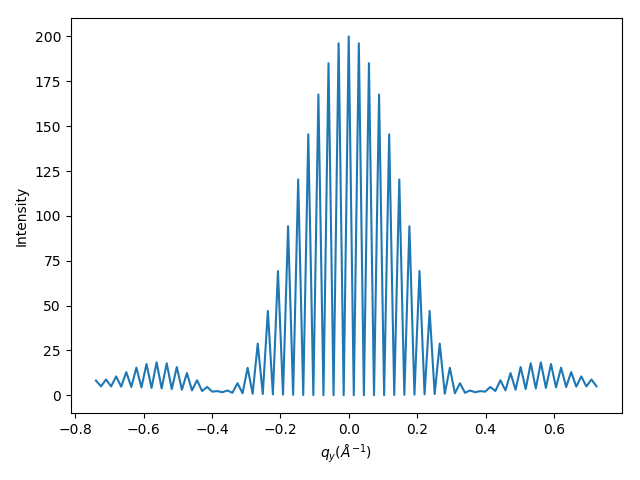
\includegraphics[width=0.45\textwidth]{constant_npores.png}
  \caption{The distance between peaks of the structure factor cross-section at
  (0, y, 1.7) is equal to the distance between pores in q-space. The first off-center
  peak of each distribution shows the fundamental frequency. The peaks that follow at 
  higher |$\mathbf{q}$| values are subharmonics. Both systems shown are in unit cells 
  with dimensions of 42.5 x 42.5 x 3.7 nm. (a) The pore-to-pore spacing was held at 
  42.5 nm. The unit cell consists of 100 total pores. The first peak is located at 
  $q_y = .148 \AA^{-1}$ which corresponds to $2\pi / .148 = 42.5 \AA$ in real space. (b)
  We placed four pores in a unit cell spaced 21.25 nm apart. The first peak appears where
  expected at $q_y = 0.0296 \AA^{-1}$ and all other peaks are separated by the same distance.
  }\label{fig:p2p_rpi}
  \end{figure}

  We quantified the peak width by fitting gaussian curves to the R-$\pi$ peak
  cross-sections and measuring ther full width at half maximum. Gaussian profiles
  appear to give the closest fit to the data (see Figure~\ref{fig:fwhm_fits}). We
  calculated all of FWHMs in ~\ref{table:perfect_size_dependence} using gaussian
  fits.

  \begin{figure}[!htb]
  \centering
  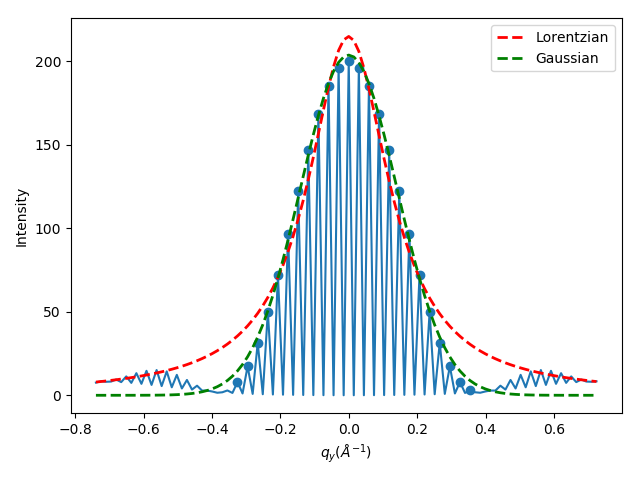
\includegraphics[width=0.5\textwidth]{fwhm_fits.png}
  \caption{The gaussian functional form more closely matches the data than the Lorentzian
  functional form. Shown is data for a perfect crystal system with 4 pores and 4 points
  per column.}\label{fig:fwhm_fits}
  \end{figure}

  The distance between pores does not affect the FWHM of the R-$\pi$ peak in
  the $q_y$ direction.  We held the size of the unit cell constant at 42.5 x 42.5
  x 3.7 nm and varied the number of pores (and consequently, the distance between
  pores). We generated error bars for the fits based on the covariance of the
  optimized fit parameters. There is no statistical difference between the
  calculated values of each FWHM. The uncertainty is lower for systems with less
  pores since there are more subharmonics available for curve fitting. The values
  of FWHM in Table~\ref{fig:perfect_size_dependence} are calculated using model
  systems with 4 pores and the same box dimensions used here. 

  \begin{table}[!htb]
  \centering
  \begin{tabular}{c c c c c}
  \toprule
  $L_z$ (\AA) & Number of Pores & Distance between Pores &  R-$\pi$ intensity & FWHM ($\AA^{-1}$) \\
  \midrule
  37          &      4            & 212.5                & 200                & 0.372 $\pm$ 0.004 \\ 
  37          &      25           & 85.0                 & 1250               & 0.371 $\pm$ 0.008 \\
  37          &      100          & 42.50                & 5000               & 0.375 $\pm$ 0.013 \\
  \bottomrule
  \end{tabular}
  \caption{We held the size of the unit cell constant at 42.5 x 42.5 x 3.7 nm and varied the
   number of pores and distance between pores. The value of FWHM is indistinguishable between
   the systems.}\label{table:randomly_displaced_columns}
  \end{table}

  The finite FWHM of perfectly crystalline systems is due to non-uniform
  ordering of the columns within the pores. Although all scatterers are aligned
  and equally spaced in the z-direction, the individual columns of scatterers are
  offset from the pore center. Therefore, there is a range of similar but
  different distances between scatter scatterers. There are many opportunities
  for constructive and destructive interference with wavelengths slightly
  different than those which contribute to the fundamental frequency. If we place
  only one column at each pore center, the FWHM becomes infinite (See
  Figure~\ref{fig:infinite_FWHM})

  \begin{figure}[!htb]
  \centering
  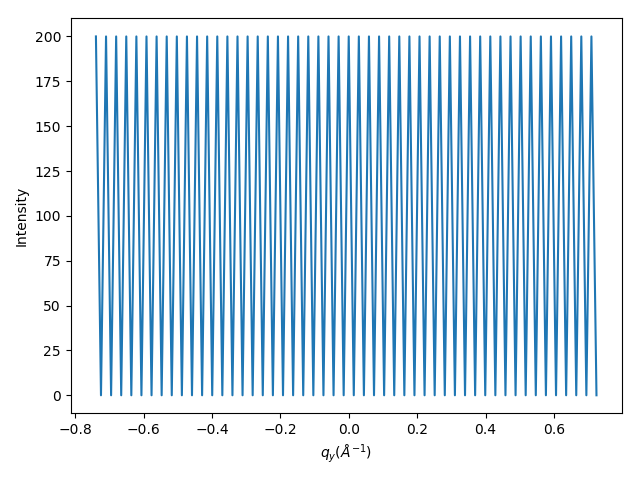
\includegraphics[width=0.5\textwidth]{one_column_per_pore.png}
  \caption{We placed one column of scatterers at each of 4 pore centers, spaced apart by
  212.5 nm. Since the y-component of the distance between all scatteres is the same in 
  all cases, subharmonics appear just as strongly as the fundamental frequency. Since the 
  intensity doesn't decay, the FWHM is infinite.}\label{fig:infinite_FWHM}
  \end{figure}

  % peaks may artifically broaden upon angle-averaging.

  The real system is far from a perfect crystal. Here we explore the influence
  of 3 sources of disorder on the intensity of R-$\pi$:
  \begin{enumerate}
  \item Random z-displacement of columns with respect to all other columns
  \item Random rotation of layers about the z-axis
  \item Thermal noise
  \end{enumerate}

  \subsection{Imperfectly aligned columns}

  We randomly aligned columns along the z-axis by adding a random displacement
  to each column of points. This simulates a system in which columns are
  uncorrelated.  We shifted coordinates where necessary so that all atoms stayed
  within the unit cell. We held the spacing between each point within each column
  remained at exactly 3.7 \AA. We created  trajectories of 1000 independent
  configurations in order to calculate the average intensity of R-$\pi$. 1000
  independent configurations gives a reasonably converged average, enough to
  observe trends.

  The intensity of R-$\pi$ is equal to the number of scatterers per
  column when we randomly displace columns with respect to each other (See
  Table~\ref{fig:randomly_displaced_columns}).  It is independent of the
  number of pores (and hence number of columns) in the system. The error 
  in the calculated intensities are comparable to the magnitude of the 
  intensity because the intensity of each configuration in the trajectory
  fluctuates so much. 

  \begin{table}[!htb]
  \centering
  \begin{tabular}{c c c c c}
  \toprule
  $L_z$ (\AA) & Points per column & Number of Pores &  R-$\pi$ Intensity\\ 
  \midrule
  14.8        &      4            & 4               & 3.98              \\
  18.5        &      5            & 4               & 5.05              \\
  37          &      10           & 4               & 10.08             \\
  14.8        &      4            & 9               & 4.06              \\
  18.5        &      5            & 9               & 4.78              \\
  37          &      10           & 9               & 10.19             \\
  14.8        &      4            & 16              & 4.01              \\
  18.5        &      5            & 16              & 4.95              \\
  37          &      10           & 16              & 9.61              \\
  \bottomrule
  \end{tabular}
  \caption{The intensity of R-$\pi$ is equal to the number of scatters in 
   each column when columns are uncorrelated.}\label{table:randomly_displaced_columns}
  \end{table}

  The $q_y$ width of R-$\pi$ is infinite when columns are randomly displaced in
  the z-direction. We attempted to measure the FWHM of the system with randomly
  displaced columns containing 4 pores and $L_z = 37$. The cross-section
  (Figure~\ref{fig:random_columns_qy}) shows non-decaying noise centered near 10,
  the same R-$\pi$ intensity in Table~\ref{table:randomly_displaced_columns}. The 
  angle averaged pattern (Figure~\ref{fig:random_columns_rzplot}) further illustrates
  the diffraction lines which characterize this type of system.

  \begin{figure}[!htb]
  \centering
  \begin{subfigure}{0.45\textwidth}
  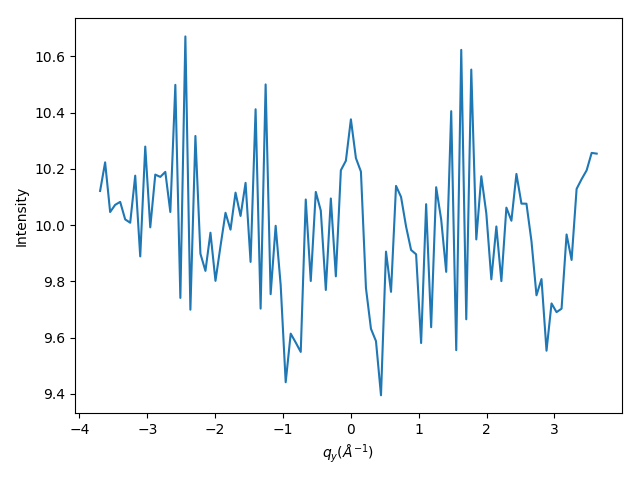
\includegraphics[width=\textwidth]{random_columns_qy.png}
  \caption{}\label{fig:random_columns_qy}
  \end{subfigure}
  \begin{subfigure}{0.45\textwidth}
  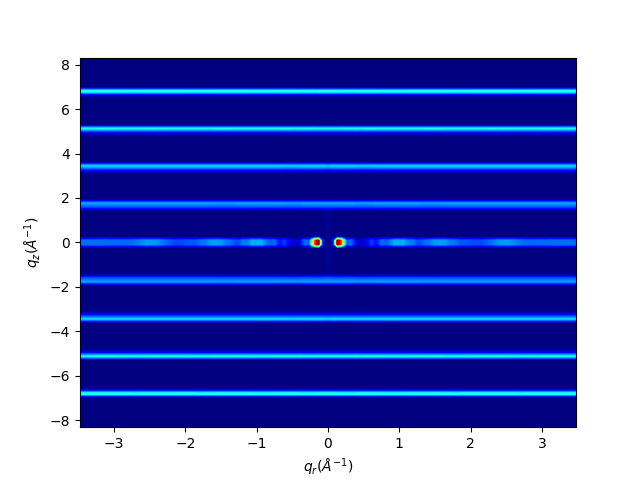
\includegraphics[width=\textwidth]{random_columns_rzplot.png}
  \caption{}\label{fig:random_columns_rzplot}
  \end{subfigure}
  \caption{}\label{fig:random_columns_rpi_width}
  \end{figure}

  \subsection{Randomly rotated layers}

  We observed the influence of correlation between layers by randomly rotating layers
  of scatterers about the z-axis. We held constant the angle, with respect to the pore
  center, between scatterers for any given layer. For examples, since there are 5 
  columns per pore, each layer is made of 5 monomers. The angle made between the two 
  vectors extending from the pore center to two adajacent scatterers in a single layer
  is 72 $\degree$ with respect to the xy plane.  

  \begin{table}[!htb]
  \centering
  \begin{tabular}{c c c c c c}
  \toprule
  $L_z$ (\AA) & Points per column & Number of Pores & Number of Atoms & R-$\pi$ Intensity & FWHM $\AA^{-1}$ \\
  \midrule
  14.8        &      4            & 4               & 80              &  80               & 0.37           \\
  18.5        &      5            & 4               & 100             &  100              & 0.37           \\
  37          &      10           & 4               & 200             &  200              & 0.37           \\
  14.8        &      4            & 9               & 180             &  180              & 0.37           \\
  18.5        &      5            & 9               & 225             &  225              & 0.37           \\
  37          &      10           & 9               & 450             &  450              & 0.37           \\
  14.8        &      4            & 16              & 320             &  320              & 0.37           \\
  18.5        &      5            & 16              & 400             &  400              & 0.37           \\
  37          &      10           & 16              & 800             &  800              & 0.37           \\
  \bottomrule
  \end{tabular}
  \caption{The intensity of R-$\pi$ is equal to the number of scatters in
   each column when columns are uncorrelated. Note that reproducing these results requires a very fine histogram, 
   and thus a much more expensive calculation. The default binning scheme (100 bins in each dimension) gives slightly
   misleading answers.}\label{table:randomly_displaced_columns}
  \end{table}

  The max intensity of R-$\pi$ and the FWHM of the $q_y$ structure factor
  cross-section at R-$\pi$ are exactly the same as those of the perfect crystal. 
 
  \subsection{Influence of Pore Radius}

  The pore radius is inversely proportional to the FWHM of systems made with
  randomly rotated layers (See Figure~\ref{fig:pore_radius}). This result is
  not extremely surprsing, although the limits of the relationship suggest 
  that a pore radius of 0 should give an infinite FWHM (supported by Figure
  ~\ref{fig:infinite_FWHM}) and an infinitely large pore radius should have 
  a zero FWHM. This result is also interesting because it suggests that one
  can measure relative pore radii using X-ray diffraction. The difficulty,
  which is associated with the phase problem, is deconvoluting the electron
  density associated with just pore entities.   

  \begin{figure}[!htb]
  \centering
  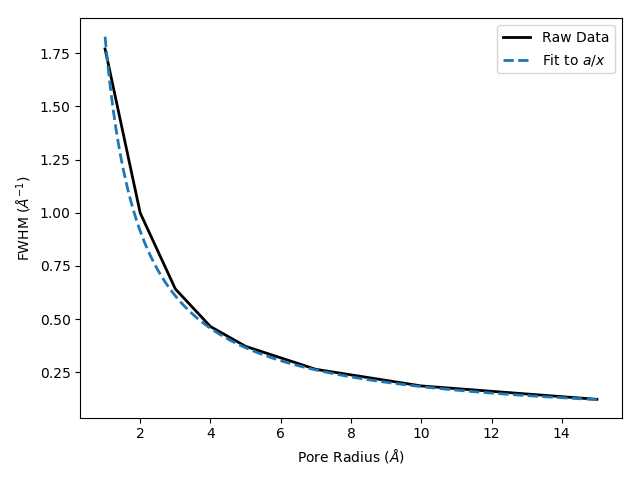
\includegraphics[width=0.5\textwidth]{pore_radius_FWHM.png}
  \caption{The FWHM decays with increasing pore radius.}\label{fig:pore_radius}
  \end{figure}

%  \begin{table}
%  \centering
%  \begin{tabular}{c c c c c c}
%  \toprule
%  $L_z$ (\AA) &   Pore Radius ($\AA^{-1}$) & FWHM ($\AA^{-1}$)  \\
%  \midrule
%  37          &      1                     &     1.770          \\
%  37          &      2                     &     0.999          \\
%  37          &      3                     &     0.642          \\
%  37          &      4                     &     0.465          \\
%  37          &      5                     &     0.372          \\
%  37          &      7	                   &     0.264          \\
%  37          &      10                    &     0.186          \\
%  37          &      15                    &     0.123          \\
%  \bottomrule
%  \end{tabular}
%  \caption{All systems contain four pores with 5 columns per pore and a unit cell
%  size of 42.5x42.5x3.7 nm. 
%  }\label{table:pore_radius}
%  \end{table}

  \subsection{The influence of thermal disorder}

  We added gaussian noise in each dimension to observe its influence on the intensity
  of R-$\pi$ and the FWHM. For the z-direction, the standard deviation of the 
  gaussian distribution is equal to a fraction of the average distance between scatterers
  in columns. In the xy-directions, the standard deviation is equal to a fraction 
  of the pore radius.

  \subsubsection{Randomly displaced columns}

  When we add noise in the z direction, the intensity of R-$\pi$ decays while the
  FWHM remains infinite.

  When we add noise in the x and y directions, R-$\pi$ has a finite peak width in its 
  $q_y$ dimension. We fit a Gaussian function to the  

  \begin{figure}
  \centering
  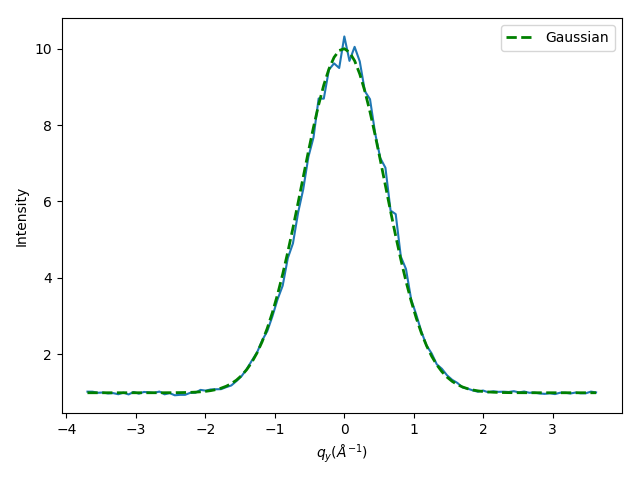
\includegraphics[width=0.5\textwidth]{random_columns_gaussian.png}
  \caption{}\label{fig:FWHM_columns}
  \end{figure}

\end{document}
